\documentclass[../main.tex]{subfiles}
\graphicspath{{\subfix{../images/}}}

\usepackage{float}

\begin{document}

\section{Materials and Methods}

This study relies on two large-scale datasets of C functions paired with x86\_64 assembly code: \textbf{ExeBench} and \textbf{The Stack}. These datasets serve as the foundation for training and evaluating data-driven decompilation models. This section details the data acquisition process, filtering strategies, structure, and known limitations.

\subsection{Dataset Overview}

We employ two complementary datasets:

\begin{itemize}
    \item \textbf{ExeBench}: A curated benchmark of executable C functions compiled at multiple optimization levels, designed for machine learning applications in compilation and decompilation \cite{armengol-estape_exebench_2022}.
    \item \textbf{The Stack}: A large-scale, permissively licensed source code repository that includes real-world C programs. While not originally intended for decompilation tasks, we compile and extract assembly representations from this dataset following a controlled pipeline \cite{kocetkov_stack_2022}.
\end{itemize}

\subsection{Data Collection and Preprocessing}

We collected examples by filterig x86 and C pairs from Exebench, and generating x86 inputs from The Stack. 
An overview of our process is illustrated by figure \ref{fig:data_gen_pipeline}

\subsubsection{ExeBench}

We process the \texttt{.jsonl.zst} files for each split (\texttt{train}, \texttt{validation}, and \texttt{test}) using \texttt{zstandard} decompression. From each JSONL entry, we extract the C source function from the \texttt{func\_def} field and the corresponding assembly from the \texttt{asm} field.

Assembly outputs include multiple compiler targets. We retain only those compiled with GCC for the x86 architecture (e.g., entries labeled \texttt{gcc\_O0}, \texttt{gcc\_Os}, \texttt{gcc\_O3}), discarding all others. This decision ensures uniformity in instruction set architecture (ISA) and aligns with common practices in decompilation research \cite{cao_boosting_2022}.

Examples are included only if they contain valid assembly code for at least one of the selected optimization levels. Most commonly, \texttt{-O0} is present, with \texttt{-Os} and \texttt{-O3} available in a substantial subset of the corpus.

\subsubsection{The Stack}

To complement ExeBench with more realistic code, we extract a subset of C source files from The Stack. These were compiled using \texttt{GCC 10.2.1} on \texttt{Debian 10 (buster)}, targeting the \texttt{x86} ISA. Compilation was performed for optimization levels \texttt{-O0}, \texttt{-Os}, and \texttt{-O3}.

Files were discarded if they failed to compile, produced empty output, or required external dependencies. Successfully compiled examples were parsed to extract assembly code and paired with the original C function. Only files with at least one valid optimization level were retained.

\begin{figure}[htbp]
\centering
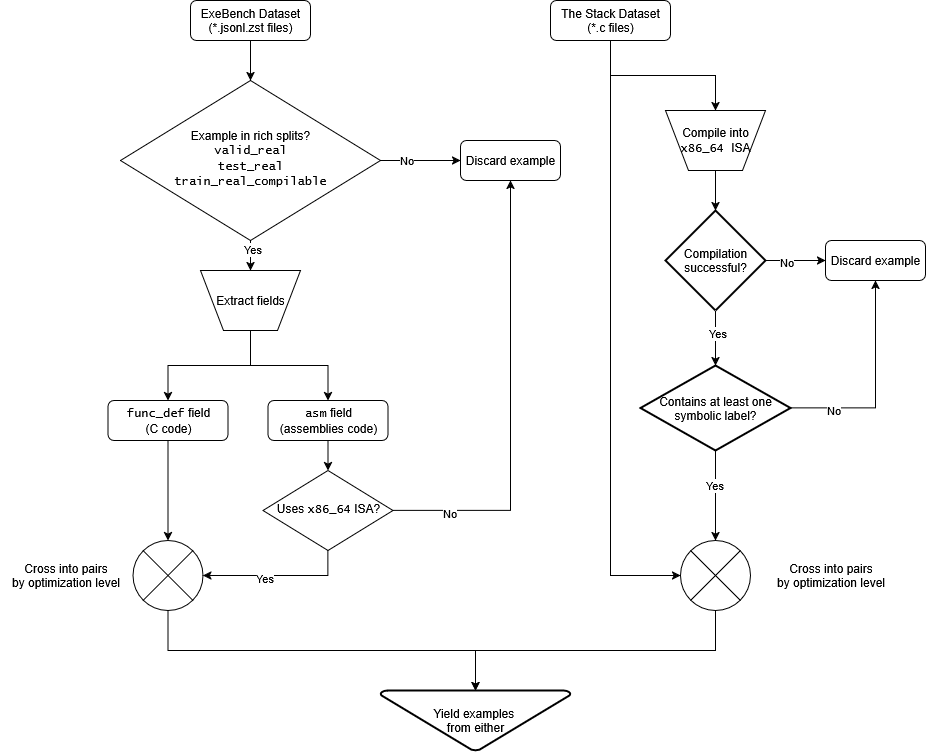
\includegraphics[width=0.5\textwidth]{images/data_gen_pipeline.png}
\caption{Data generation and preprocessing pipeline overview}
\label{fig:data_gen_pipeline}
\end{figure}

\subsection{Dataset Structure}

Each valid example is stored as a JSON object with the following structure:

\begin{itemize}
    \item \texttt{c}: the original C function code.
    \item \texttt{asm}: a dictionary mapping optimization levels (e.g., \texttt{O0}, \texttt{Os}, \texttt{O3}) to the corresponding x86 assembly code.
\end{itemize}

Examples are organized into directories according to their respective splits: \texttt{train/}, \texttt{valid/}, and \texttt{test/}. Assembly outputs are normalized to remove formatting artifacts, improving downstream processing without altering semantics.

\subsection{Dataset Composition}

The final dataset composition is summarized below, distinguishing between the ExeBench and The Stack corpora. Each example is considered valid if it contains a successfully compiled C function paired with its corresponding x86 assembly representation for at least one of the selected optimization levels (\texttt{-O0}, \texttt{-Os}, \texttt{-O3}).

\begin{itemize}
    \item \textbf{ExeBench}:
    \begin{itemize}
        \item Approx.\ 20,950 total examples in the full dataset.
        \item All examples contain \texttt{O0}; around 70\% also include \texttt{Os} and/or \texttt{O3}.
    \end{itemize}
    \item \textbf{The Stack}:
    \begin{itemize}
        \item Approx.\ 120,000 compiled examples considered initially.
        \item A filtered subset of 348 valid examples was selected for evaluation purposes.
        \item Over 85\% of retained examples include multiple optimization levels.
    \end{itemize}
\end{itemize}

Tables~\ref{tab:stack_dist} and~\ref{tab:exebench_dist} provide a breakdown of optimization levels and examples across splits for both datasets.

\vspace{1em}

\begin{table}[H]
\centering
\caption{Distribution of processed examples from The Stack by split and optimization level}
\label{tab:stack_dist}
\begin{tabular}{lccc}
\toprule
\textbf{Optimization Level} & \textbf{Train} & \textbf{Validation} & \textbf{Test} \\
\midrule
O0 & 93 & 12 & 11 \\
Os & 93 & 12 & 11 \\
O3 & 93 & 11 & 12 \\
\midrule
\textbf{Total} & \textbf{279 (80.17\%)} & \textbf{35 (10.06\%)} & \textbf{34 (9.77\%)} \\
\bottomrule
\end{tabular}
\end{table}

\vspace{1em}

\begin{table}[H]
\centering
\caption{Distribution of processed examples from ExeBench by split and optimization level}
\label{tab:exebench_dist}
\begin{tabular}{lccc}
\toprule
\textbf{Optimization Level} & \textbf{Train} & \textbf{Validation} & \textbf{Test} \\
\midrule
O0 & 5582 & 698 & 698 \\
Os & 5588 & 699 & 698 \\
O3 & 5587 & 699 & 699 \\
\midrule
\textbf{Total} & \textbf{16757 (80.00\%)} & \textbf{2096 (10.00\%)} & \textbf{2095 (10.00\%)} \\
\bottomrule
\end{tabular}
\end{table}


\subsection{Limitations}

Despite the careful design and preprocessing of the datasets, several practical limitations must be acknowledged.

\textbf{Storage space} was a significant constraint. The total size of the dataset exceeded 60~GB, which can be challenging to manage in constrained computing environments or when reproducing results. The final dataset was deliberately capped to ensure accessibility and feasibility for training and evaluation.

Additionally, the \textbf{data preparation pipeline} required substantial \textbf{processing time}. Larger-scale processing---such as compiling all C files available in The Stack---was deemed infeasible within our compute budget, leading us to restrict the final corpus.

A further limitation involves the \textbf{compilability} of real-world source code. A significant number of C files from The Stack could not be compiled due to syntax errors, reliance on platform-specific headers, unresolved macros, or missing dependencies. These cases were automatically filtered out. Although this process ensured that all included samples were syntactically and semantically valid, it introduces a selection bias that favors simpler or more portable code.

Lastly, \textbf{example length} posed a constraint from a model architecture perspective. Transformer-based language models operate with fixed-length input windows. In our case, the DistilGPT \cite{sanh2019distilbert} variant used during experimentation is limited to a context window of approximately 1024 tokens. Some valid examples---especially those containing large functions or multiple optimization levels---exceeded this limit and could not be processed end-to-end. Although we considered filtering out these longer samples, doing so would bias the dataset toward short and trivial functions, reducing its representativeness. As such, we retained these examples in the dataset, with the understanding that future work may require truncation, segmentation, or hierarchical modeling strategies to accommodate them.

\subsection{Model}

\begin{itemize}
  \item \textbf{Problem formulation:}  
    Assembly-to-C decompilation is cast as a \emph{causal autoregressive} language-modeling task. At each timestep \(t\) the DistilGPT2 model predicts the next token \(w_t\) in the target C sequence conditioned on the full assembly prompt and all previously generated C tokens:
    \[
      p(x) \;=\;\prod_{t=1}^{T} p_\theta(w_t \mid w_{<t})\,.
    \]

  \item \textbf{Architecture and pretrained weights:}  
    We fine-tune \emph{DistilGPT2}, a 6-layer, 82 M-parameter distilled variant of GPT-2, chosen for its moderate footprint and compatibility with our compute/storage constraints.

  \item \textbf{Input:}  
    Prompts employ a multi-turn template (implemented in \texttt{model\_loading.py}), for example:
    \begin{verbatim}
<|system|> You are a C decompiler model.
<|user|> Decompile this x86_64 assembly:
<|tool_start|> [x86 code] <|tool_end|>
    \end{verbatim}
    Special tokens \texttt{<|tool\_start|>} / \texttt{<|tool\_end|>} clearly delimit the assembly block.

  \item \textbf{Output:}  
    After the \texttt{<|assistant|>} marker, the model generates the C source code:
    \begin{verbatim}
<|assistant|> [Predicted C code]
    \end{verbatim}
    Only these C tokens are unmasked and contribute to training.

  \item \textbf{Loss function:}  
    We use \emph{categorical cross-entropy} with token-level masking (implemented in \texttt{model\_evaluation.py}). Prompt and assembly tokens receive a sentinel label (–100) and are excluded; only C-token positions incur loss:
    \[
      \mathcal{L} = -\!\!\sum_{t \in \mathcal{T}_C}\log p_\theta(w_t \mid w_{<t}).
    \]

  \item \textbf{Metrics:}  
    A custom \texttt{BatchDecompilerMetrics} class collects:
    \begin{itemize}
      \item \emph{Token classification:} accuracy, precision, recall, F1-score.
      \item \emph{Language modeling:} cross-entropy loss, perplexity.
    \end{itemize}
\end{itemize}

\subsection{Training}

\begin{itemize}
  \item \textbf{Sampling and splitting:}  
    We stratify by dataset origin (ExeBench vs.\ The Stack) and by optimization level (O0, Os, O3). Each stratum is split 80/10/10 for train/validation/test, preserving the distribution of compile-time flags across splits.

  \item \textbf{Hyperparameters:}  
    Configured via a \texttt{create\_training\_args()} helper:
    \begin{itemize}
      \item \emph{num\_train\_epochs}: user-specified (5–10).  
      \item \emph{learning\_rate}: 5e-5 with 100 warmup steps.  
      \item \emph{weight\_decay}: 0.01.  
      \item \emph{gradient\_accumulation\_steps}: 8 for effective large batches.  
      \item \emph{fp16}: enabled when CUDA is available.  
      \item \emph{eval\_strategy}: “steps,” evaluating every 5\% of total steps.  
    \end{itemize}

  \item \textbf{Data collation:}  
    We employ \texttt{DataCollatorForLanguageModeling} (with \texttt{mlm=False}) for causal LM batching, ensuring correct padding and attention masks.

  \item \textbf{Compute environment:}  
    Training runs under SLURM (see \texttt{test\_pretrained.slurm}) on GPU nodes:
    \begin{itemize}
      \item 2 × NVIDIA A100 80 GB per node, 64-core Intel Xeon CPUs, 16 GB RAM/core.  
      \item PyTorch, Hugging Face Transformers, Accelerate, CuPy.  
      \item Memory monitoring hooks log both host and CUDA usage (\texttt{model\_training.py}).  
      \item Checkpointing: resume from existing checkpoint if detected; save every 5\% steps with a total‐limit of 1.
    \end{itemize}

  \item \textbf{Metrics collection and visualization:}  
    The \texttt{collect\_training\_metrics()} function parses the trainer’s history to produce:
    \begin{itemize}
      \item \emph{Loss vs.\ steps/epochs} plots (training/validation).  
      \item \emph{Token metrics} over time (precision, recall, F1, accuracy).  
      \item \emph{LM metrics} (perplexity and cross-entropy).
    \end{itemize}

  \item \textbf{Memory optimizations:}  
    The system logs virtual memory and CUDA allocations each step; uses gradient accumulation and mixed-precision to fit large effective batch sizes on limited GPU memory.
\end{itemize}


\end{document}
